\section{Cloud Architektur}
In diesem Kapitel wird auf die verwendete Infrastruktur Architektur in \ac{AWS} eingegangen. Die nachfolgende Abbildung gibt einen Überblick wie die einzelnen Komponenten miteinander kommunizieren und voneinander abhängen. Drüber hinaus werden einige Gründe für die Auswahl der Services aufgezeigt.

\begin{figure}[H]
    \centering
    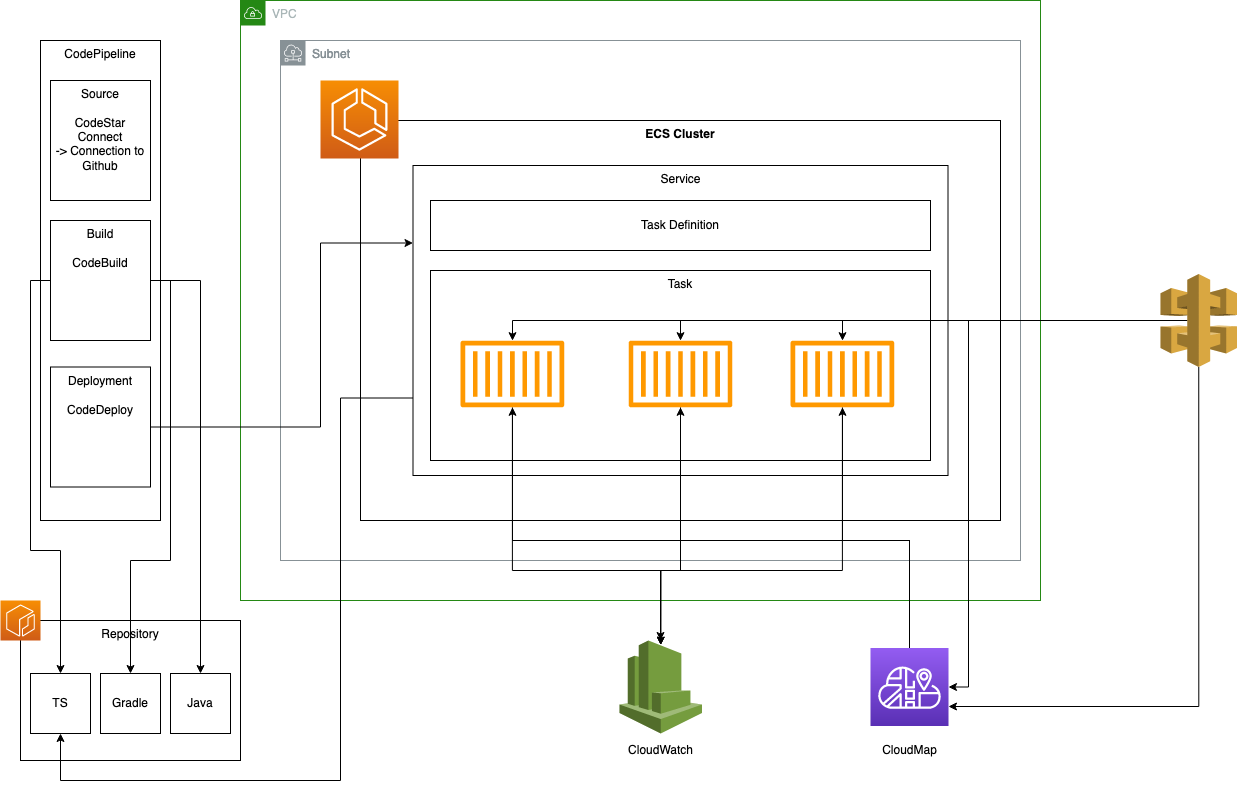
\includegraphics[width=\textwidth]{aws_architecture.png}
    \caption{Architekturentwurf für die AWS-Services}
    \label{fig:CloudArchitektur}
\end{figure}

Ziel ist es, die Anwendung auf Containern zu deployen. Dazu wird \ac{ECS} mit einem \gls{Fargate}-Worker eingesetzt zur Bereitstellung eines Clusters mit serverless Containern. Innerhalb des Clusters ist in einer \textit{Taskdefinition} festgelegt, wie viele Container gestartet werden sollen und die \textit{Task} selbst, in welcher die Container bereitgestellt werden.

Das \ac{ECS} Cluster selbst befindet sich innerhalb eines von einer \ac{VPC} bereitgestellten Subnetz. Erreichbar sind die einzelnen Container über ein \textit{\ac{API} Gateway}, welches auf die IP-Adressen innerhalb des Subnetzes verweist. Die Adressen der Container werden in \textit{CloudMap} gespeichert und der Betrieb dieser mit \textit{CloudWatch} überwacht.

Neben dem \ac{ECS} Cluster wird als weiterer Service \textit{\gls{CodePipeline}} eingesetzt. Dieser Kombiniert die Services \textit{CodeStar}, \textit{CodeBuild} und \textit{CodeDeploy}. \textit{CodeStar} stellt hierbei eine Verbindung zu \gls{GitHub} her, wo der Anwendungscode abgelegt ist. \textit{CodeBuild} erzeugt ein Abbild der Anwendung in einem Container und legt diesen in \ac{ECR} ab. \textit{CodeDeploy} deployt die aktuellste Version der Anwendung aus \ac{ECR} in das Cluster.